%
\hsection{Relationship Diagrams}%
\FloatBarrier%
%
\begin{figure}%
\centering%
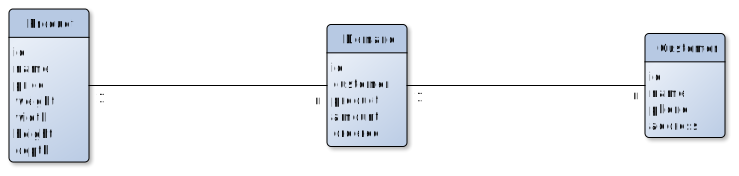
\includegraphics[width=0.9\linewidth]{\currentDir/factoryDbErd}%
\caption{An \pgls{ERD} for our factory \pgls{db}, hand-drawn with \yEd. %
You will learn more about that in \cref{sec:conceptualSchemaDesign}.}%
\label{fig:factoryDbErd}%
\end{figure}%
%
\begin{figure}%
\centering%
%
\subfloat[][%
To get to the \pgls{ERD} view, we click on \menu{Tools} and then \menu{Relationships}.%
\label{fig:factoryLibreOfficeBaseErd1Open}%
]{\tightbox{\includegraphics[width=0.49\linewidth]{\currentDir/factoryLibreOfficeBaseErd1Open}}}%
%
\floatSep%
%
\subfloat[][%
An \pgls{ERD} view of the tables in our \db\ appears. %
It is a bit cluttered, so we drag the tables around and resize them a bit.%
\label{fig:factoryLibreOfficeBaseErd2overview}%
]{\tightbox{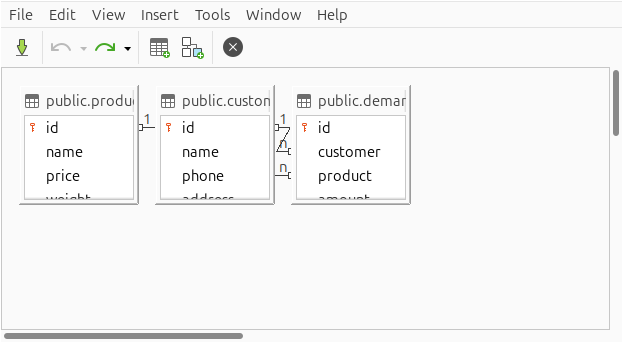
\includegraphics[width=0.49\linewidth]{\currentDir/factoryLibreOfficeBaseErd2overview}}}%
%
\floatRowSep%
%
\subfloat[][%
The \pgls{ERD} now looks very clean and illustrates the relationships between the tables in our \db.%
\label{fig:factoryLibreOfficeBaseErd3overviewRearranged}%
]{\tightbox{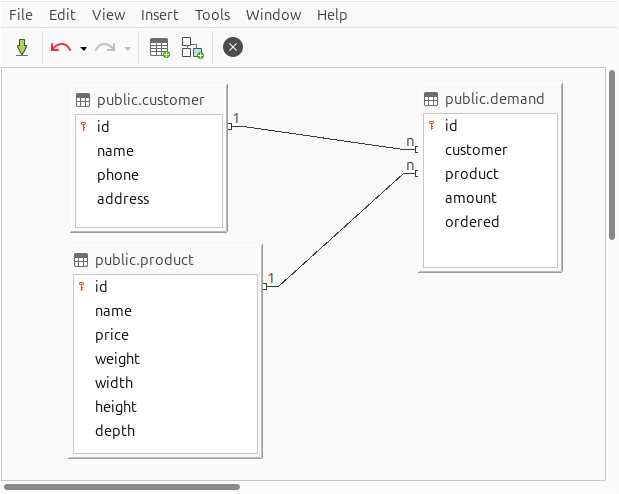
\includegraphics[width=0.7\linewidth]{\currentDir/factoryLibreOfficeBaseErd3overviewRearranged}}}%
%
%
\caption{Viewing an \pgls{ERD} of the tables and their relations in our \db\ in \libreofficeBase.}%
\label{fig:factoryLibreOfficeBaseERD}%
%
\end{figure}%
%
An important tool in \db\ development are \glsreset{ERD}\pglspl{ERD}.
\pglspl{ERD} are normally used when we design a abstract (conteptual) model of a \db.
They are visual representations of the objects and the relationships between them.
It makes a lot of sense to first create a model of the real-world objects or information that we want to store in the \db\ before implementing the \db\ using \sql.
The modeled objects can then be mapped to tables and the relationships could become foreign key relationships.

In \cref{fig:factoryDbErd}, we present a small \pgls{ERD} that sketches the objects that make up our factory \db.
As you can see, all three object types and their attributes are illustrated.
The lines linking them present their relationships.
Here we see that one customer~(and product) entity can be linked to an arbitrary number of demand entities.
Each demand entity, on the other hand, is linked to exactly one customer~(and product) entity.
We can construct the \db\ structure based on this design.
In \cref{sec:conceptualSchemaDesign}, we will in-depth discuss this approach to conceptual \db\ modeling.

In our example \db, however, we just directly started with the table design in \sql.
We wanted to see action as quickly as possible and disregarded any concern about efficient design.
This example is not about fancy stuff, it is about exploring the world of \pglspl{db}.

Let's say that we did indeed design a \db\ based on entities modeled in a \pgls{ERD}.
The \db\ is created via \sql\ commands.
The tables and thei foreign key relationships then correctly represent the model painted as \pgls{ERD}.
Then, the information in the \pgls{ERD} is also present in the \db.
It is reflected the structure of the tables and the foreign keys.
If this is true, then we should be able to reconstruct the \pgls{ERD} at least partially from a \db.
Of course, we cannot reconstruct the semantics, i.e., the meaning behind the relationships and objects.
But we can well reconstruct the objects and relationships on a purly syntactical level.
Actually, we can do that so quickly that we can always work with an \pgls{ERD}-based representation of our \db.

\libreofficeBase\ can do that.
We therefore first open our dokument \textil{factory.odb} using \libreofficeBase.
To connect with the \db, we will have to enter the password \textil{superboss123}.
We open the menu~\menu{Tools} and then click on \menu{Relationships}, as illustrated in \cref{fig:factoryLibreOfficeBaseErd1Open}.
This opens a very cluttered diagram view.
This view includes all three tables that we designed in our \db, but in~\cref{fig:factoryLibreOfficeBaseErd2overview} they are not neatly arranged.

We can click on them, though, and drag them around.
We can also drag the bottom edges of the tables and expand them.
After some re-arranging, we get indeed a very nice overview on our \db\ in \cref{fig:factoryLibreOfficeBaseErd2overview}.

We can see that the \sqlil{id} columns are the primary keys of the tables, because they are marked with key icons~\libreOfficeBaseKey.
Furthermore, we see that each \sqlil{id} value in table \sqlil{customer} can be used in $n$~records as \sqlil{customer} value in table~\sqlil{demand}.
The same holds for each \sqlil{id} value in table \sqlil{product}, which can be stored in $n$~records as \sqlil{product} value in table~\sqlil{demand}.
$n$~here stands for \inQuotes{arbitrarily often.}

This \pgls{ERD} is a really overview on the structure of our \db.
And it can automatically be generated for us by the \libreofficeBase\ \pgls{GUI}.
If our \db\ was more complex, with more tables and relationships, this illustration could be quite helpful.
Imagine that we join a department of an organization as the new \pgls{dba}.
Imagine you get to work on an existing \db.
Sadly, there is no documentation available.
All we can do is to access the \dbms\ and try to figure out how the \db\ works via \sql.
Well, if we would connect with \libreofficeBase\ to the \dbms, we could at least get a quick and comprehensive overview on the structure of the \db, what tables exist, and how they are related.%
%
\FloatBarrier%
\endhsection%
%
